\documentclass[journal]{IEEEtran}

\usepackage{blindtext}
\usepackage{cite}
\usepackage{graphicx}
\usepackage{array}
\usepackage{color}
\usepackage{tabularx}
\usepackage{epsfig}
\usepackage{amsmath}
\usepackage{amssymb}
\usepackage{bm}
\usepackage{wasysym}
\usepackage{circuitikz}
\usepackage{float}
\usepackage{algorithm}
\usepackage{algorithmic}

\usetikzlibrary{arrows,shapes,calc,positioning}

\newcommand{\myscope}[2]
{\draw[thick,rotate=#2] (#1) circle (12pt)
(#1) ++(-0.35,-0.1) --++ (0.3,0.3) --++ (0,-0.3) --++(0.3,0.3) --++(0,-0.3);}

\begin{document}

\title{CSCE 221 \\ Problem Set 19}

\author{Jacob~Purcell,~\IEEEmember{Texas~A\&M,~Student}}

\maketitle
\section{}
\begin{figure}[h!]
    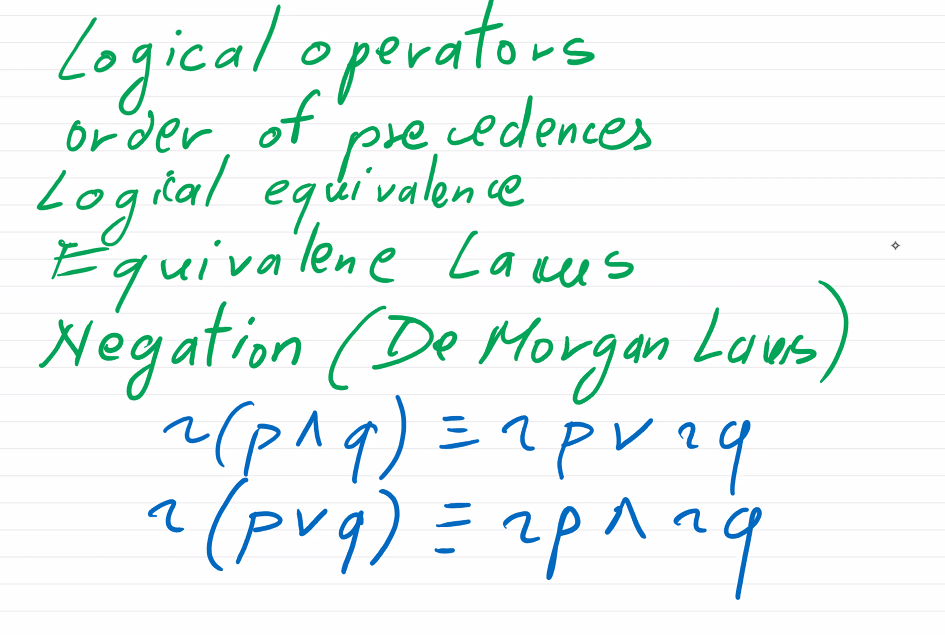
\includegraphics[scale = 1]{Capture.png}
    \caption{Huffman Code of the given table.}
\end{figure}

\section{}
If the frequencies are sorted then they are already in heap order within their storage container, 
which is best implemented as a priority queue. Dequeue the first two nodes, add them together and 
construct a new tree, inserting the compound node with the dequeued nodes as its children. Check both trees
for minimum value to construct new parent in a similar manner to how the second tree was constructed.
 Repeat until first two trees are empty, thee third tree is the final result. This requires $\frac{3N}{2}$
operations (full pass through first tree, at most $\frac{N}{2}$ operaitons in second tree.) which is $\boxed{O(N)}$.
\end{document}
